\documentclass{article}
\usepackage{polski}
\usepackage[utf8]{inputenc}
\usepackage{graphicx}
\usepackage{subcaption}
\usepackage{latexsym}
\usepackage{geometry}
\usepackage{float}

\title{Sprawozdanie z ćwiczeń laboratoryjnych nr 8\\Tablice z haszowaniem}
\author{Kacper Kafara\\nr grupy 9\\śr. 14:40}
\date{14 maja 2020}
\pagenumbering{gobble}
\begin{document}
\maketitle
\newpage

\section{Zadanie}
Zgodnie z "Instrukcją do ćwiczeń laboratoryjnych":
\begin{itemize}
	\item Porównanie czasów wykonania oraz liczby \emph{kolizji} w algorytmach haszowania otwartego dla różnych danych wejściowych. 
	\item Pomiar czasu wykonania algorytmu haszowania łańcuchowego dla różnych danych wejściowych.
\end{itemize}

\section{Metodologia}
\begin{itemize}
	\item Do pomiaru czasu wykonania algorytmów wykorzystana została funkcja \emph{clock\_t clock()}. 
	\item Pomiar czasu wykonania algorytmów opierał się na: 
	\begin{itemize}
		\item wygenrerowaniu bazy danych (o zadanym rozmiarze $n$) złożonej z rekordów \emph{[name, number]}
		\item wygenerowaniu sekwencji $k$ zapytań (add / remove / get) oraz numerów rekordów do których odnosi się poszczególne zapytanie
		\item 100-krotnym pomiarze czasu wykonania wszystkich 3 algorytmów (każdy pomiar dla tej samej bazy danych, ale za każdym razem generowana nowa $k$ elementowa sekwencja zapytań)
		\item za czas wykonania algorytmu przyjęta została średnia arytetyczna ze wszystkich 100 prób. 
	\end{itemize}
	\item Liczba kolizji to podobnie $\lfloor srednia-arytmetyczna-z-liczby-kolizji \rfloor$.
\end{itemize}

\section{Rezultaty}
\indent 
W dalszej części sprawozdania zamieszona została seria wykresów czasu wykonania $t$ $([t] = s)$ poszczególnych algorytmów haszowania w zależności od liczby zapytań przy ustalonej wielkości bazy danych oraz - w przypadku haszowania otwartego - także wykresy ilości kolizji od ilości zapytań. W lewym górnym rogu każdego z wykresów znajdziemy rozmiar bazy danych $n$ dla którego były wykonywane pomiary. Na osi poziomej liczba zapytań $k$. Dla każdego $n$ zostały wybrane 3 liczby zapytań: znacznie mniejsza od rozmiaru bazy, nieco mniejsza niż rozmiar bazy oraz przewyższająca rozmiar bazy. 

\subsection{Haszowanie otwarte}
\indent
Kolorami oznaczone rodzaje haszowania otwartego. 

\begin{figure}[H]
	\centering
	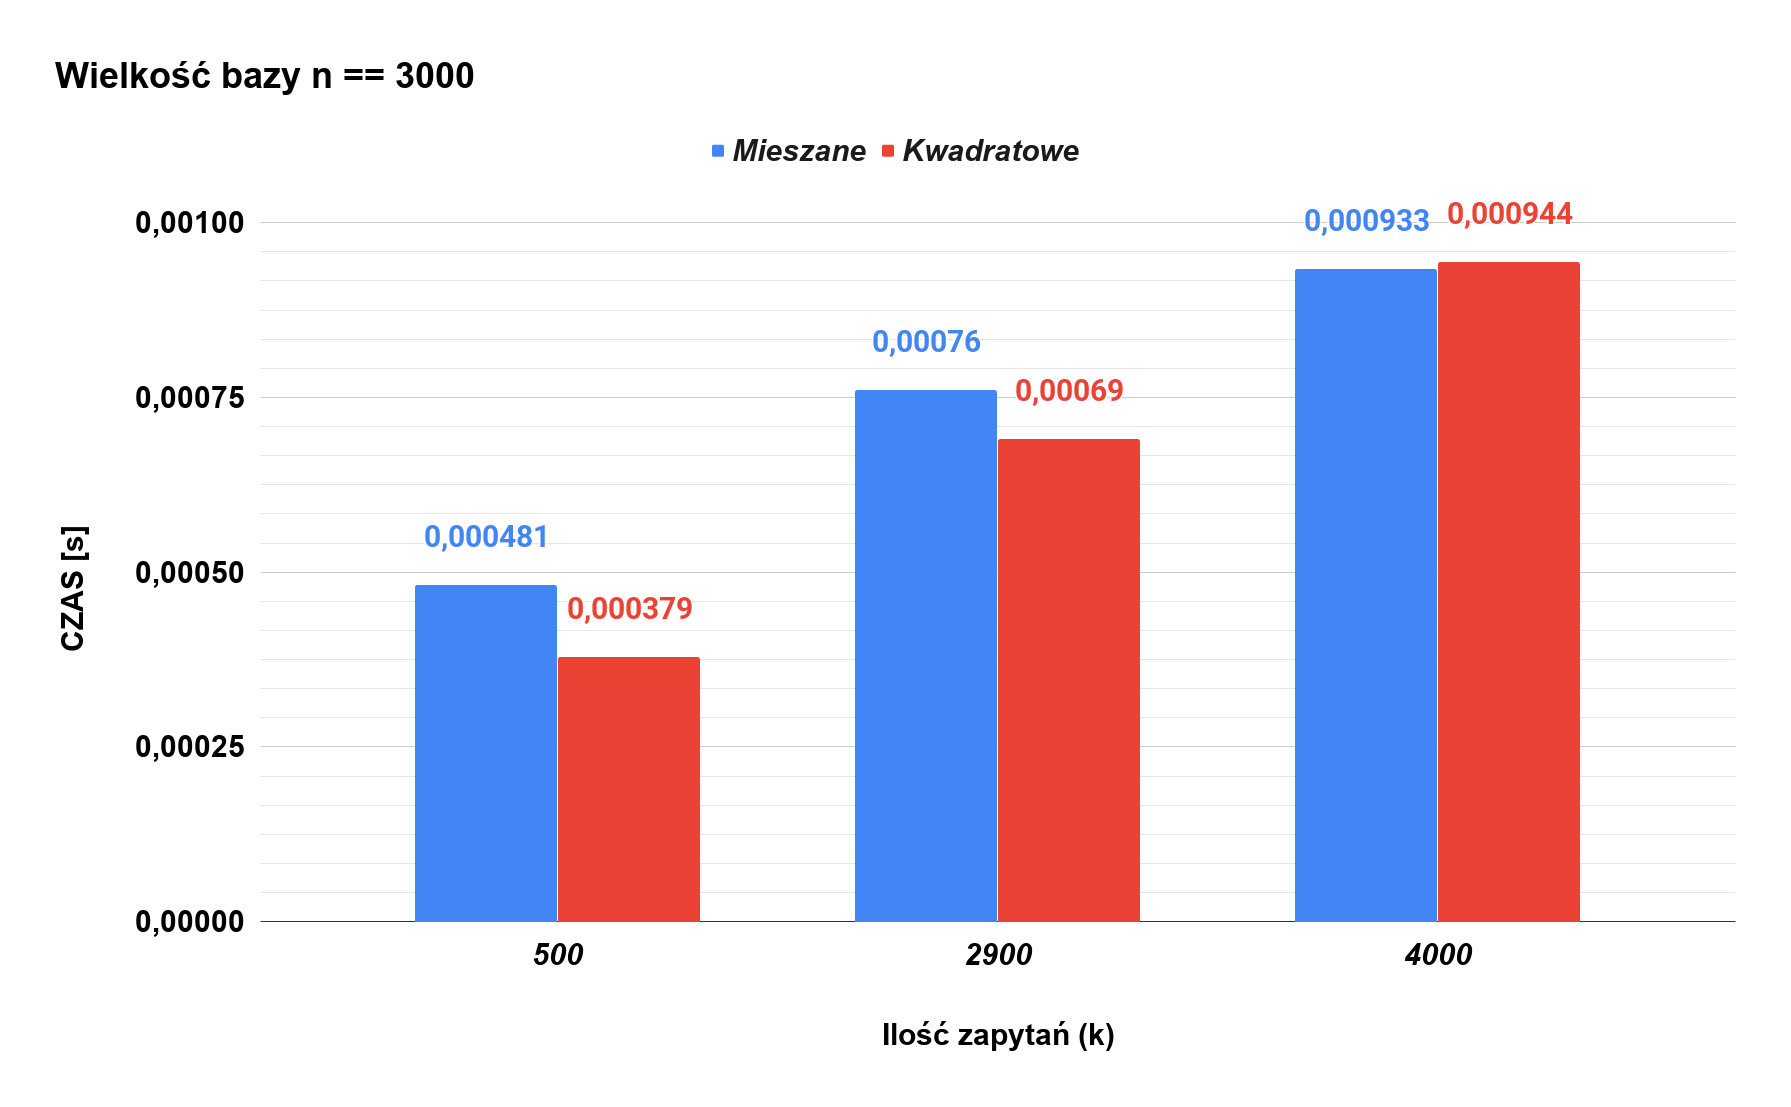
\includegraphics[scale=0.22]{mkn3k.png}
	\caption{czas(ilość\_zapytań), $n = 3000$}
	\label{fig:mkn3k}
\end{figure}
\begin{figure}[H]
	\centering
	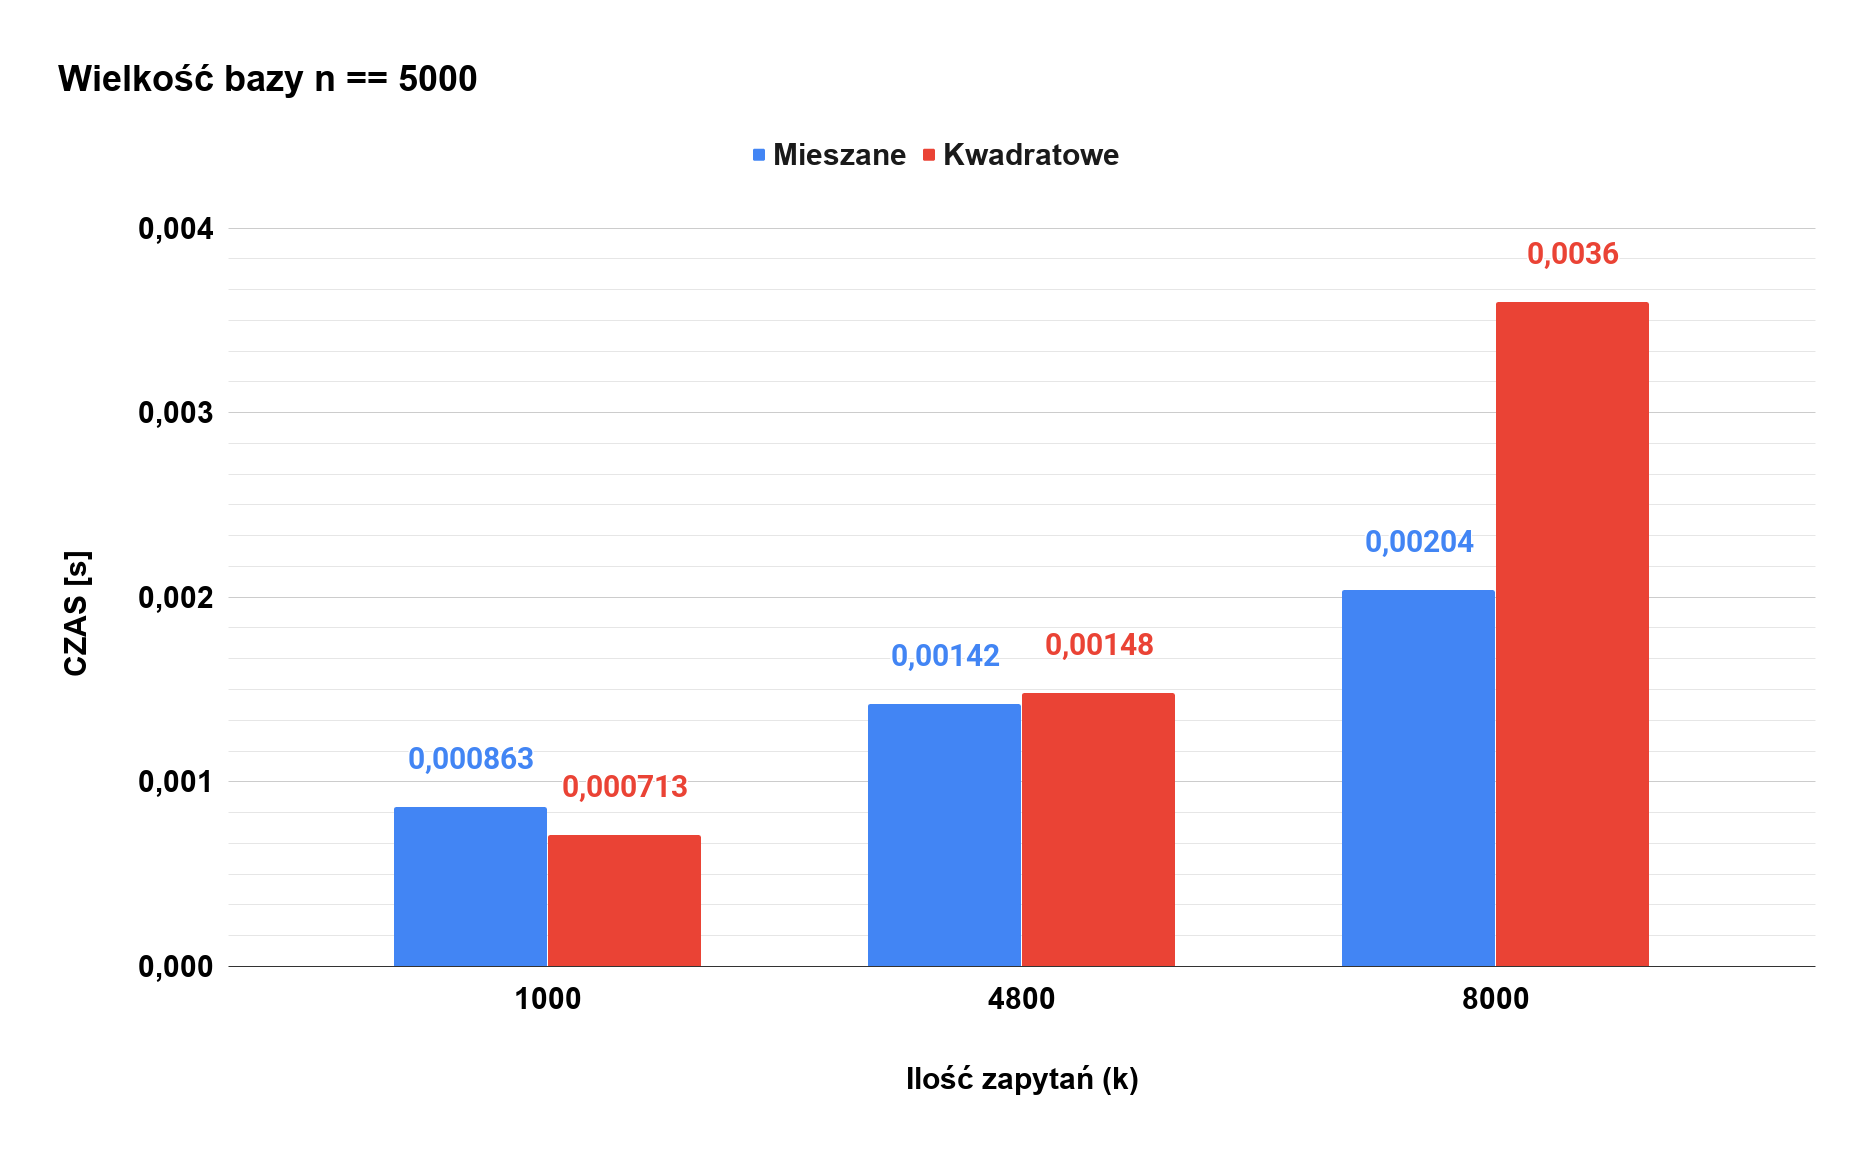
\includegraphics[scale=0.21]{mkn5k.png}
	\caption{czas(ilość\_zapytań), $n = 5000$}
	\label{fig:mkn5k}
\end{figure}
\begin{figure}[H]
	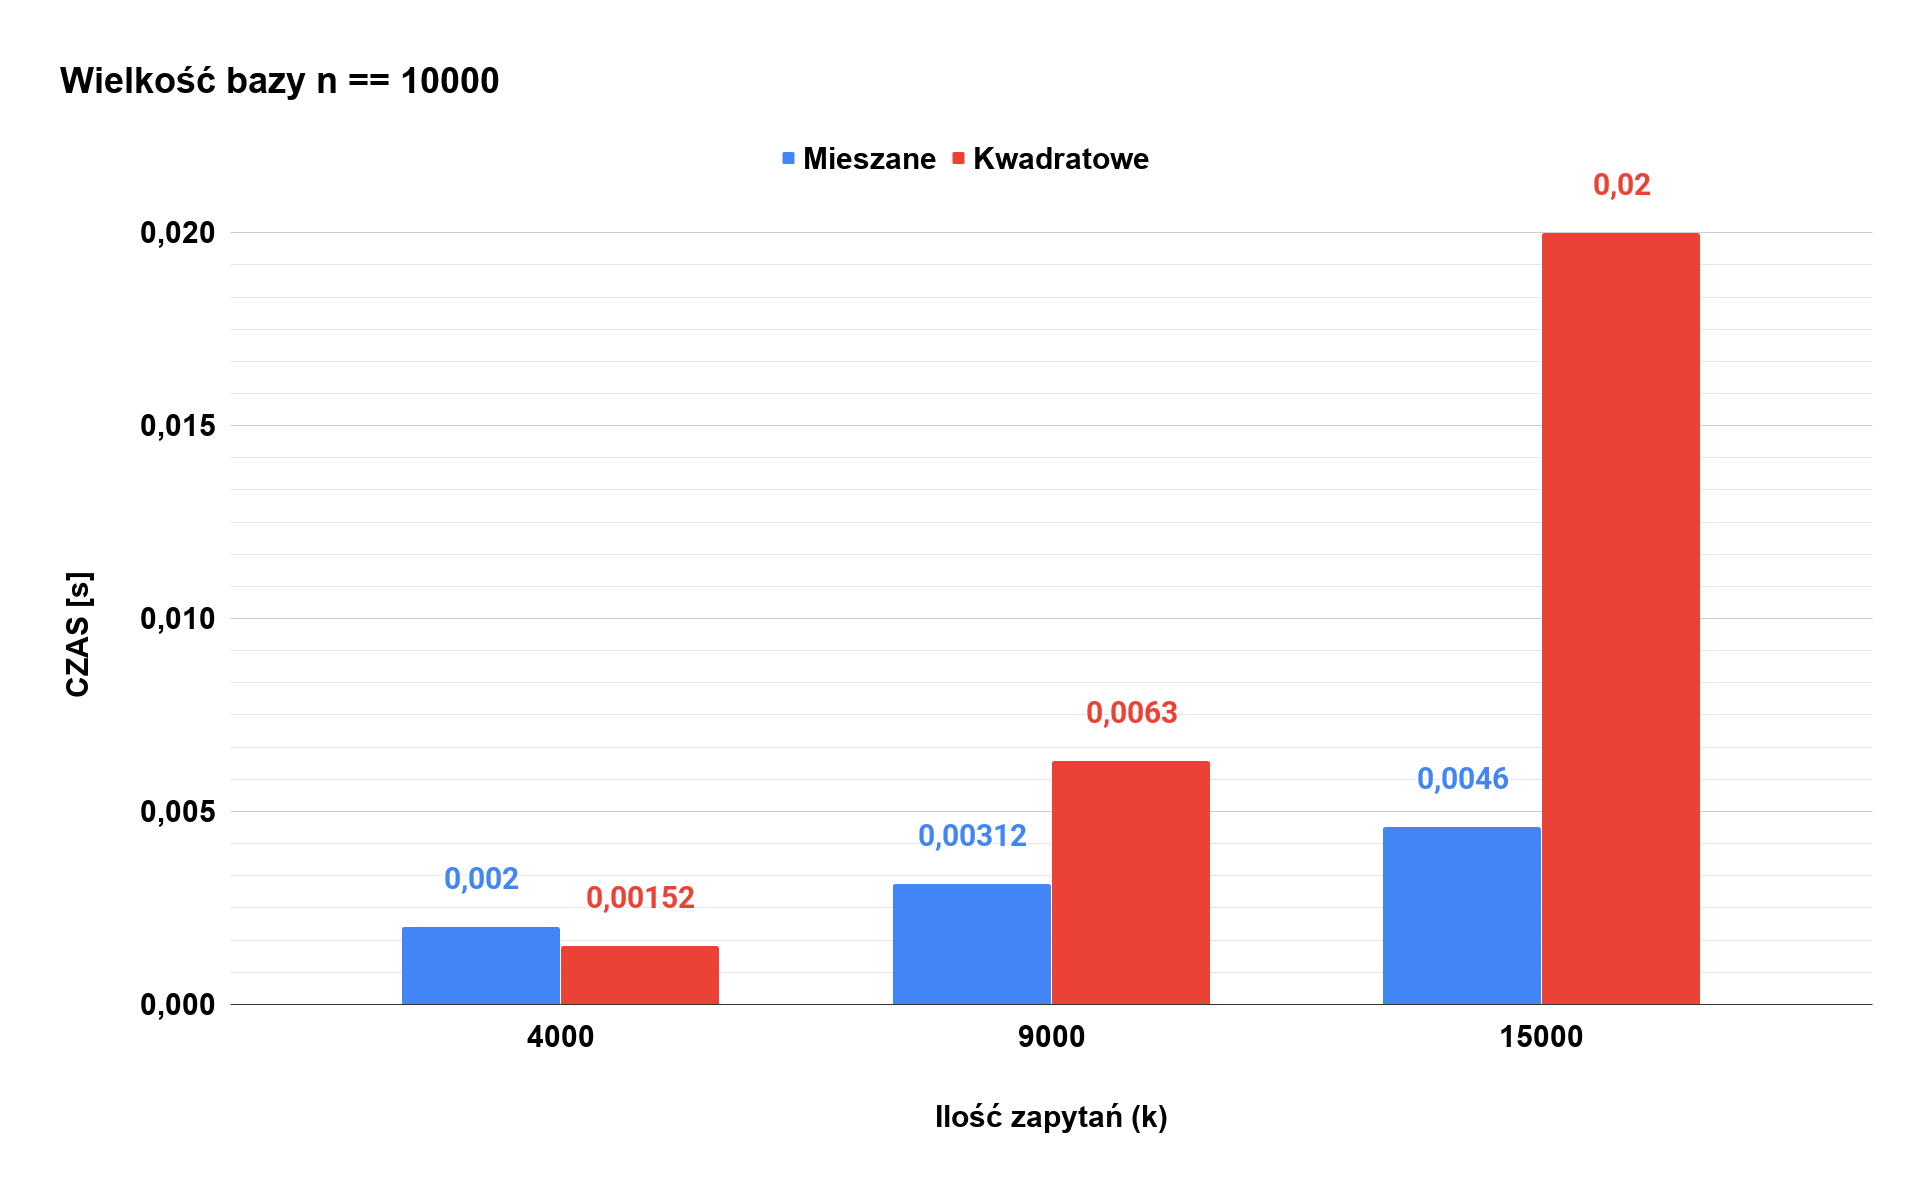
\includegraphics[scale=0.22]{mkn10k.png}
	\caption{czas(ilość\_zapytań), $n = 10000$}
	\label{fig:mkn10k}
\end{figure}
\begin{figure}[H]
	\centering
	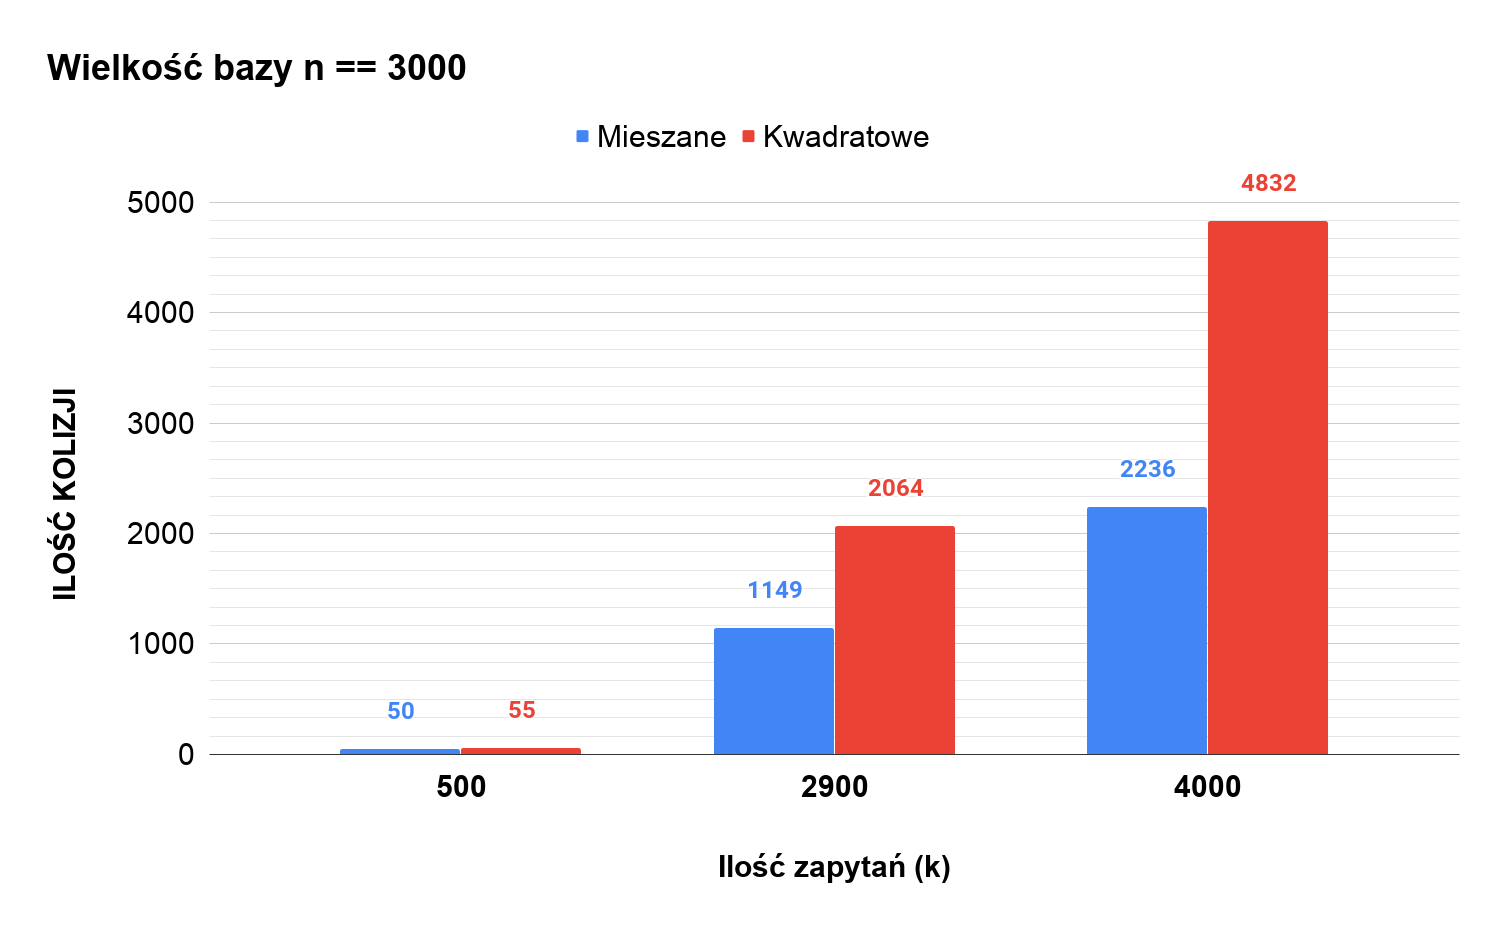
\includegraphics[scale=0.24]{kolizjen3k.png}
	\caption{ilość\_kolizji(ilość\_zapytań), $n = 3000$}
	\label{fig:kolizjen3k}
\end{figure}
\begin{figure}[H]
	\centering
	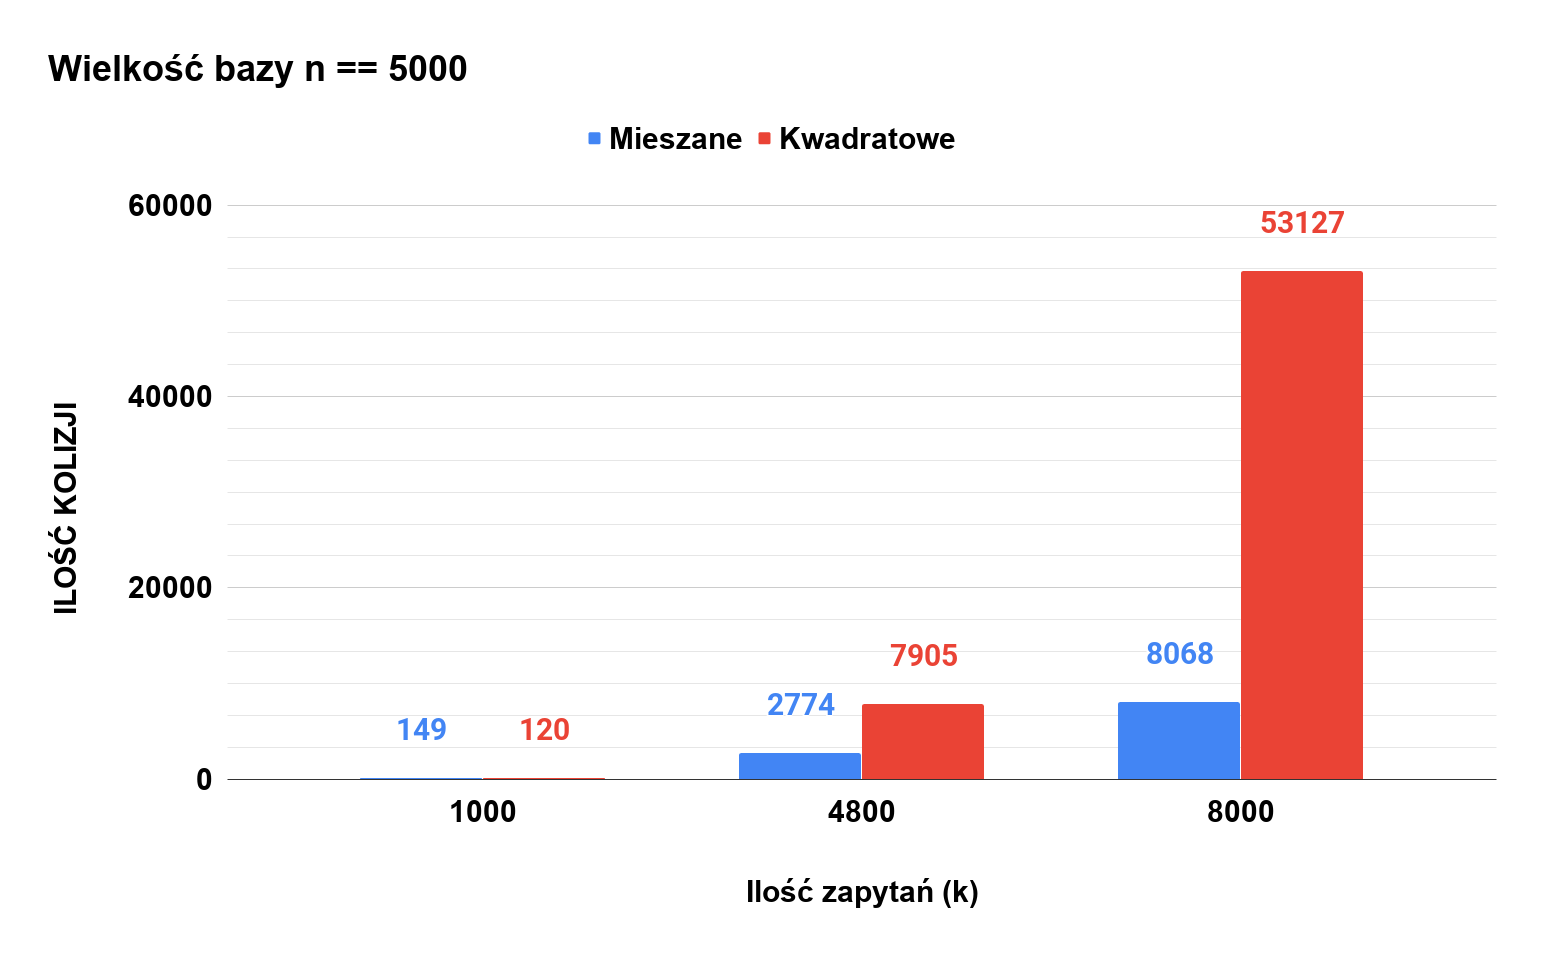
\includegraphics[scale=0.25]{kolizjen5k.png}
	\caption{ilość\_kolizji(ilość\_zapytań), $n = 5000$}
	\label{fig:kolizjen5k}
\end{figure}
\begin{figure}[H]
	\centering
	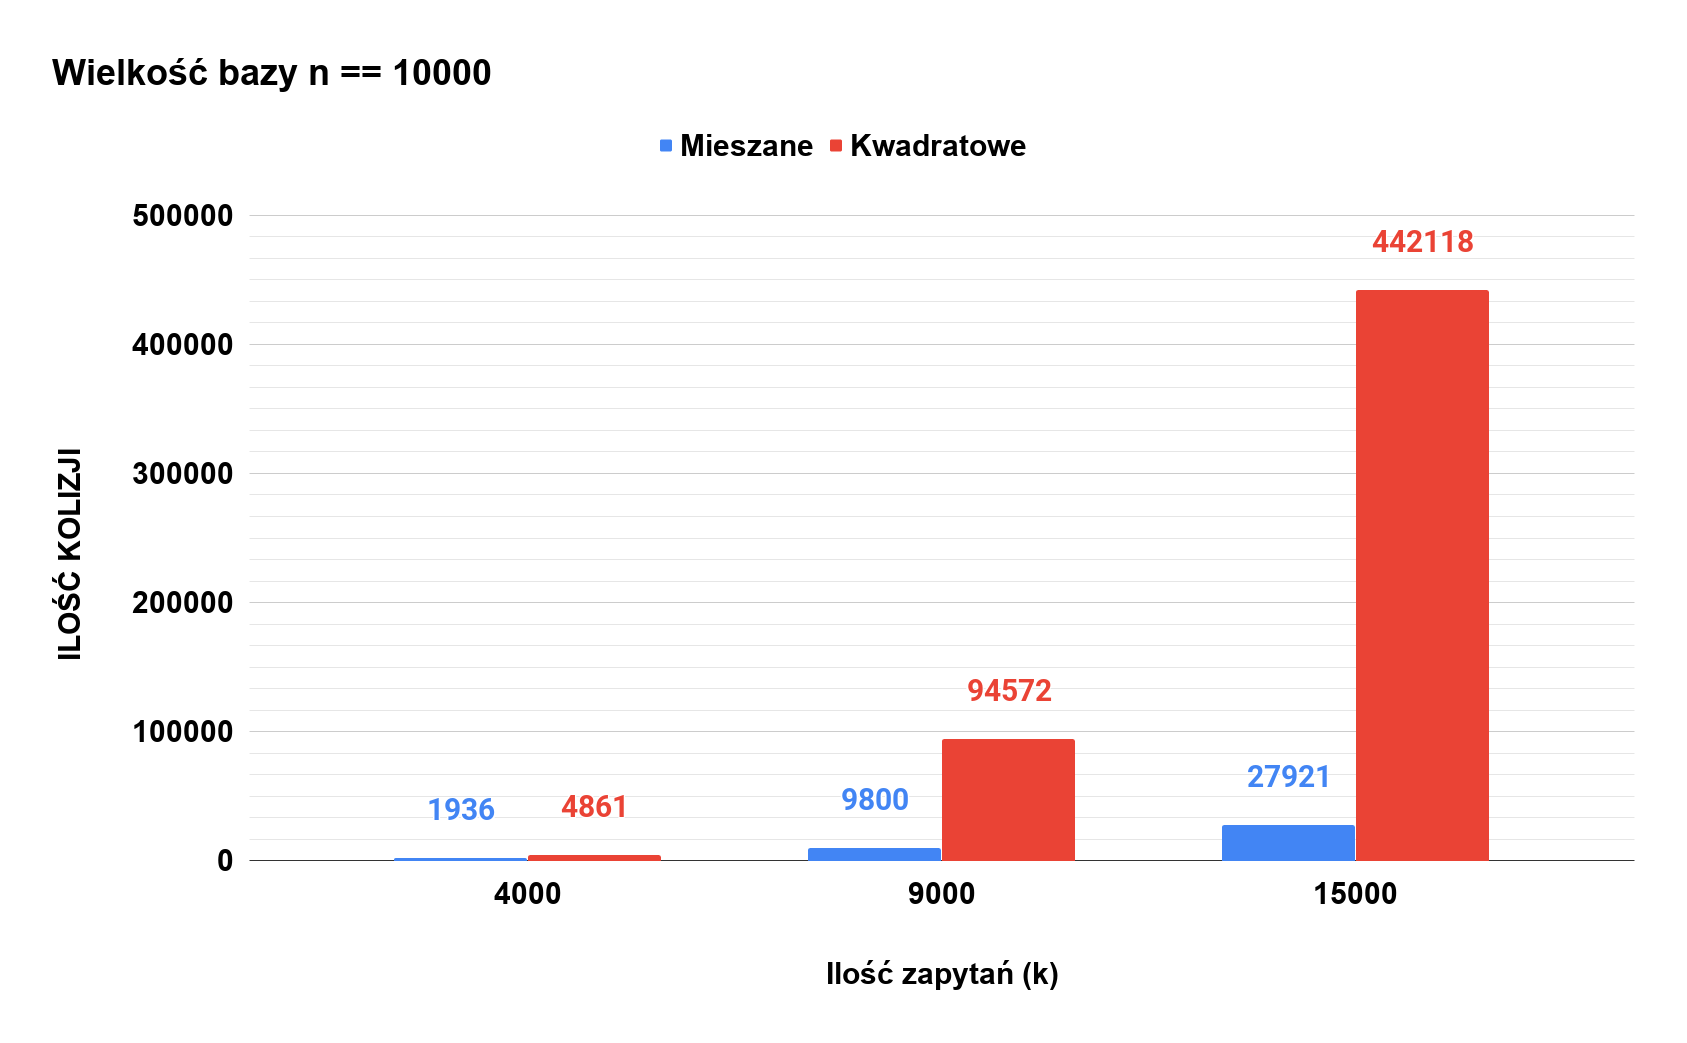
\includegraphics[scale=0.24]{kolizjen10k.png}
	\caption{ilość\_kolizji(ilość\_zapytań), $n = 10000$}
	\label{fig:kolizjen10k}
\end{figure}



\newpage

\subsection{Haszowanie łańcuchowe}
\begin{figure}[H]
	\centering
	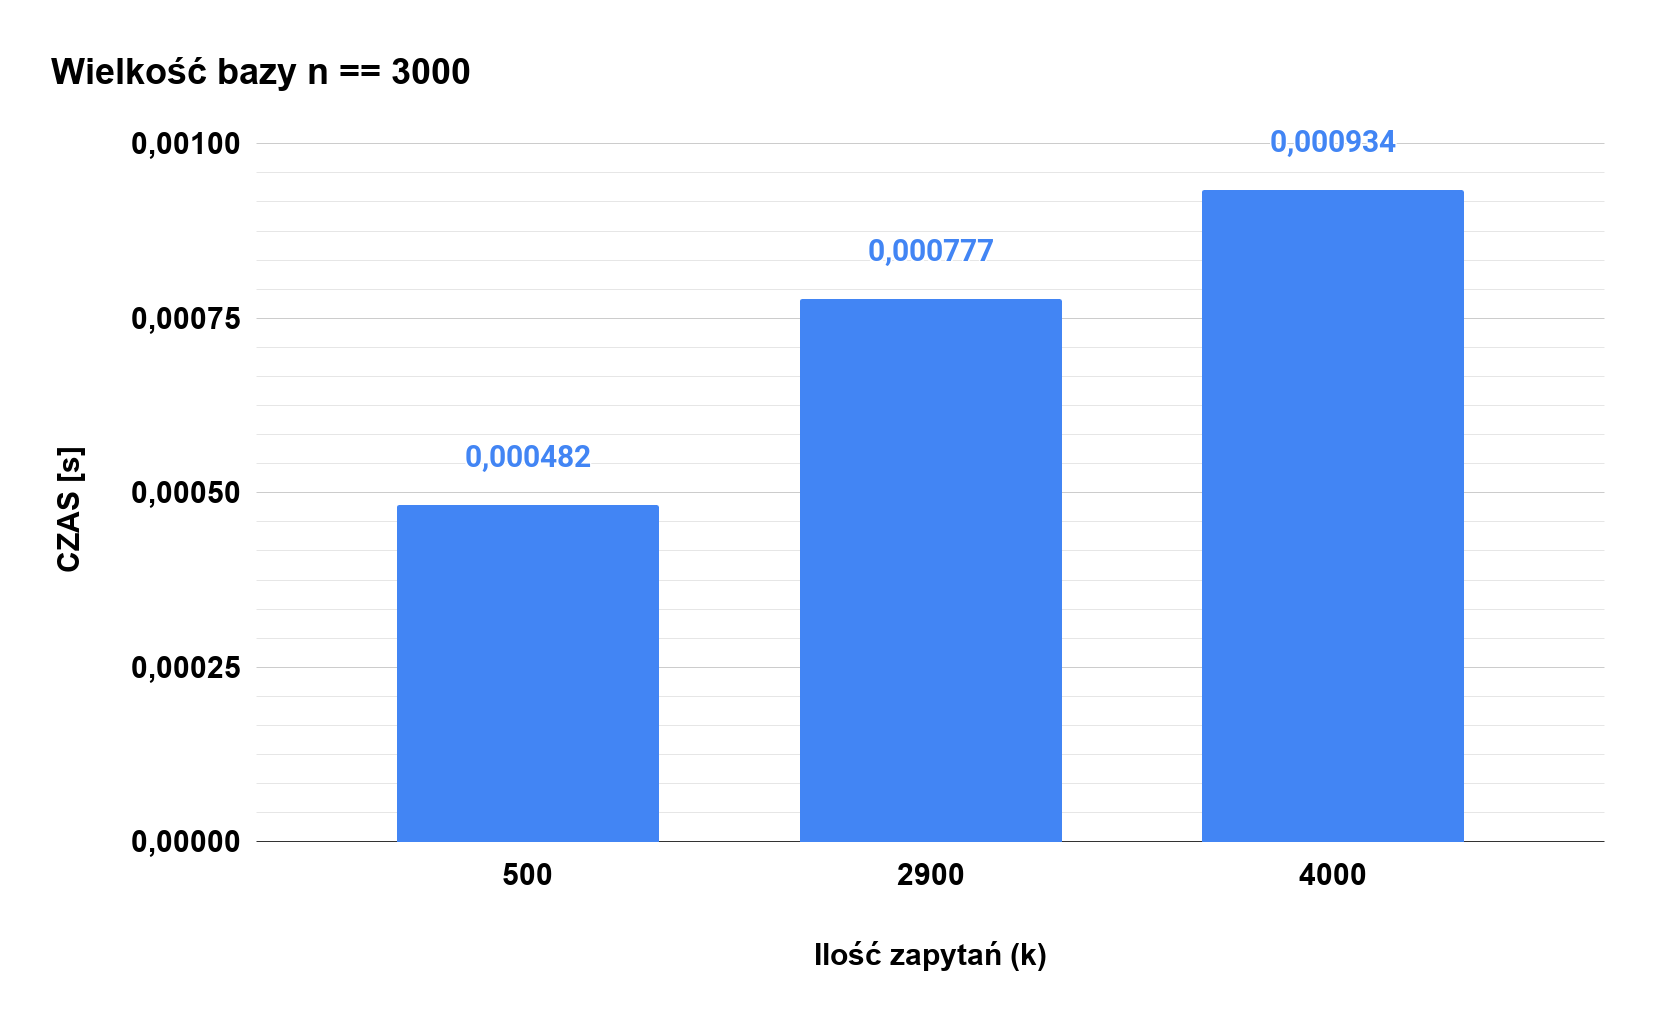
\includegraphics[scale=0.22]{ln3k.png}
	\caption{czas(ilość\_zapytań), $n = 3000$}
	\label{fig:ln3k}
\end{figure}

\begin{figure}[H]
	\centering
	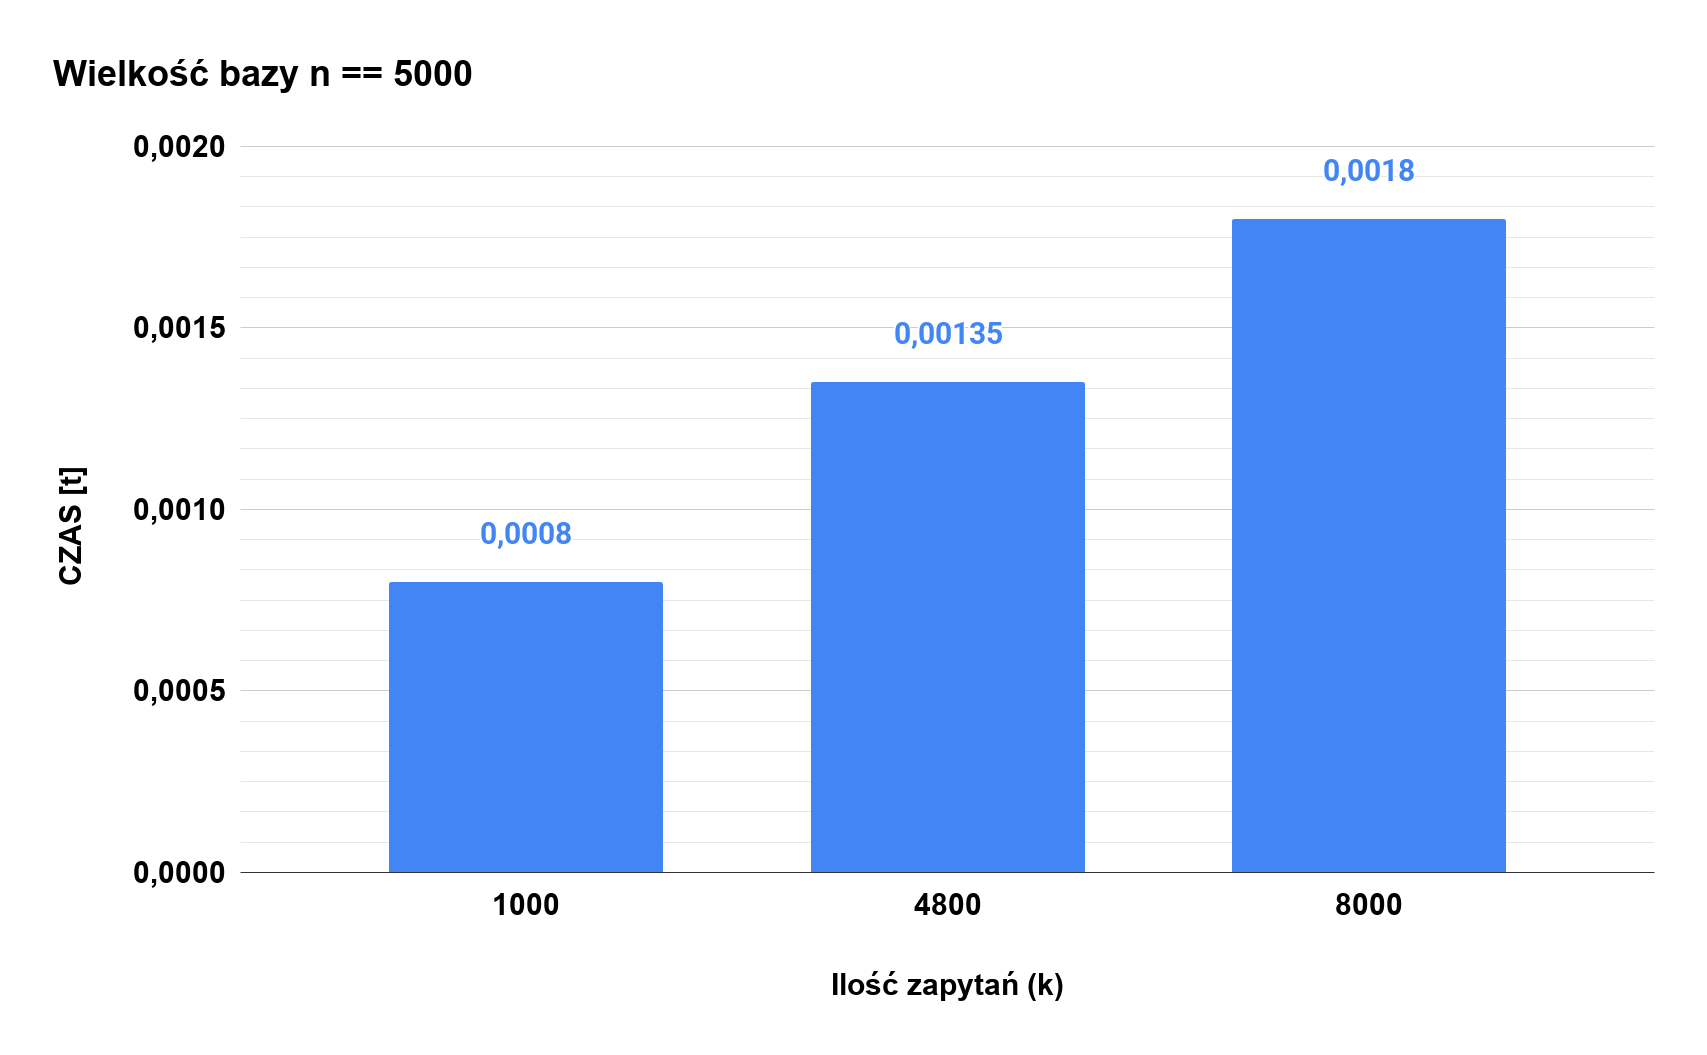
\includegraphics[scale=0.22]{ln5k.png}
	\caption{czas(ilość\_zapytań), $n = 5000$}
	\label{fig:ln5k}
\end{figure}

\begin{figure}[H]
	\centering
	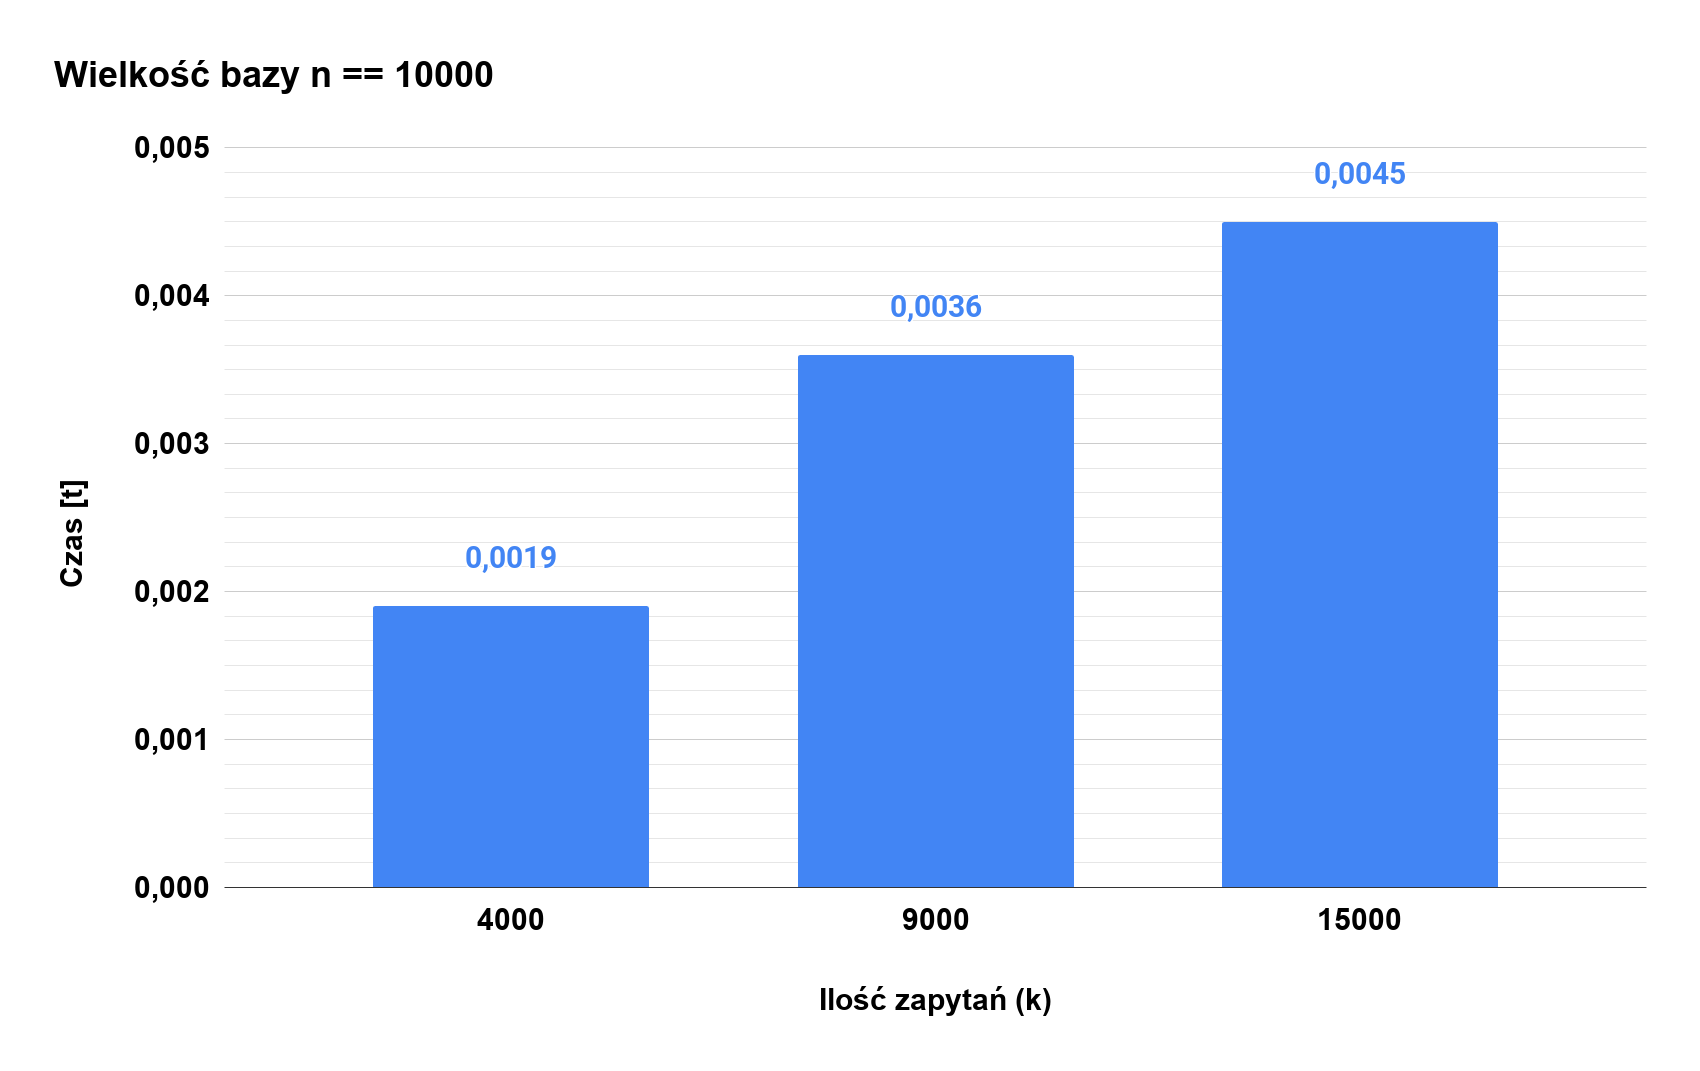
\includegraphics[scale=0.22]{ln10k.png}
	\caption{czas(ilość\_zapytań), $n = 10000$}
	\label{fig:ln10k}
\end{figure}

\section{Wnioski}
\subsection{Haszowanie otwarte}
\begin{itemize}
	\item Metoda z adresowaniem kwadratowym wydaje się być szybsza dla stosunkowo małych baz danych oraz liczby zapytań niższej niż mocy całego uniwersum kluczy. Rzadko jednak wiemy jak liczny jest zbiór wszystkich możliwych kluczy $\Rightarrow$  metoda z adresowaniem mieszanym obciążona jest mniejszym ryzykiem gwałtownego wzrostu czasu wykonania.
	\item Adresowanie mieszane daje znacznie bardziej stabilne rezultaty niż adresowanie kwadratowe.
	\item Adresowanie mieszane prowadzi do znacznie mniejszej ilości kolizji (a w takim razie mamy mniej tracenia czasu na dodatkowe obliczenia), szczególnie gdy ilość zapytań zbliża się do mocy uniwersum kluczy lub go przewyższa. 
	\item Widzimy, że adresowanie kwadratowe w pewnych przypadkach z pewnością nie działa w czasie stałym. (Można popatrzeć na bardzo zmienny stosunek czasu wykonania algorytmu od ilości zapytań, szczególnie dla $k >> n$.
\end{itemize}
\subsection{Haszowanie łańcuchowe}
\begin{itemize}
	\item Dla losowych (pseudolosowych) danych daje czasy zbliżone do adresowania mieszanego. 
	\item Jeżeli popatrzymy na stosunek czasu wykonania algorytmu do liczby zapytań to możemy zauważyć że jest on w przybliżeniu stały ($\simeq 0,24 * 10^{-6}$)dla różnych $n$ i $k$, co odróżnia ten algorytm od algorytmu z adresowaniem kwadratowym. 
	\item Z poprzedniego punktu wynika, że algorytm działa w spodziewanym czasie stałym. 
\end{itemize}
%\subsection{Haszowanie łańcuchowe}
%xCOKOLWIEK
\end{document}